\chapter {Analyse du monde de l'édition vidéo professionnel}

\minitoc \mtcskip \newpage


\paragraph{}

%désolé Thibault mais je ne comprends pas bien cette première phrase: à  quoi peut-on s'attendre exactement ??Le montage vidéo professionnel est un domaine très vaste, et l'on peut
s'attendre à ce que les besoins auxquels doivent répondre les logiciels
permettant de produire les différents types d'œuvres audiovisuelles
varient fortement en fonction du type de contenu. Afin d'étudier les
possibilités d'avenir des logiciels libres dans ce domaine, il nous
faut définir, pour en connaître les différents besoins:

\begin{itemize} \setlength{\itemsep}{2mm}

  \item {les cas d'utilisation (plus communément appelées use cases
    \index{use cases})}

  \item {les fonctionnalités qui en découlent}

\end{itemize}


\paragraph{}

Nous allons donc définir les principa%les utilisations en fonction
des différents types de productions audiovisuelles et ainsi en déduire
les fonctionnalités nécessaires pour répondre à ces %utilisations.

\paragraph{}

Ensuite %nous analyserons la base commune des fonctionnalités nécessaires à
la %réalisation de ces différents types de production.  Pour finir nous verrons %s'il
%existe une diversité dans les besoins, et essayerons de trouver les fonctionnalités
qui sont propres à chaque type de production. Cette première analyse a
pour but de clarifier les besoins des professionnels afin de déterminer
par la suite quels sont ceux auxquels les logiciels libres répondent
déjà, ceux auxquels on peut prétendre répondre dans un futur proche,
et ceux qui sont hors du scope actuel des technologies libres.

\newpage

\section{Les bases de l'édition vidéo}

\paragraph{}

Tout d'abord, il est évident que, pour qu'un logiciel de montage
puisse répondre aux besoins des professionnels, ses fonctionnalités
basiques de l'édition vidéo non linéaire doivent être couvertes.
Cette partie a pour but de définir quelles sont ces fonctionnalités,
et de les expliquer succinctement:

\subsection{Définition des termes techniques}

\paragraph {}

Du fait de l'importance des termes suivant pour la compréhension de
ce document, il est nécessaire qu'ils soient définis au sein même
de celui-ci.

\paragraph{Les Footages}

Les footages correspondent à toutes les sources brutes qui ont été
enregistrées et a partir desquelles% le monteur va créer le rendu
final de l'œuvre audiovisuelle.

\paragraph{Les clips}

Les clips correspondent dans les faits à un footage édité (retouche
des couleurs, modification de la durée, ajout d'effets\ldots) par le
monteur afin de l'utiliser dans le contexte précis d'une œuvre finale.

\subparagraph{Les templates}

Dans l'édition video, on parle de template pour définir un moule de
montage.  Il permet au monteur de monter très rapidement des oeuvres
en s'assurant que le rendu rentre dans un cadre défini précédemment.

\paragraph{Colorimétrie (retouche des couleurs)}

En édition vidéo la colorimétrie est l'art de retoucher les couleurs,
les étalonner au travers des différents clips.

\begin{wrapfigure}{r}{0.5\textwidth}

   \vspace{-20pt}

    \begin{center}

      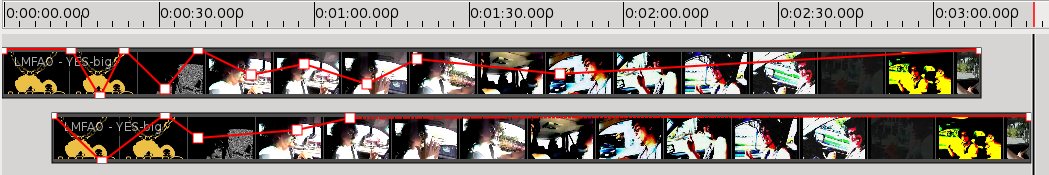
\includegraphics[width=0.48\textwidth]{images/keyframecurves}

    \end{center}

   \vspace{-30pt} \caption{Les keyframes} \vspace{-10pt} \label{Yes}

\end{wrapfigure}

\paragraph{Les keyframes}

Les keyframes définissent le %début et la fin d'une
animation, en particulier dans le cadre d'effet,%?? de texte en mouvement
au dessus d'une vidéo\ldots

\paragraph{Speed control et time remmaping}

Le speed control permet de modifier la vitesse de lecture d'un clip
dans la timeline (ralentir ou accélérer). Le time remapping est une
technique avancée de speed control, et permet de changer la vitesse de
lecture de partie de clip, et ainsi d' accélérer ou de ralentir des
parties d'un même clip. Cette technique est couplée au keyframes afin
d'obtenir le résultat souhaité.

\paragraph{Gestion des Footages}

Un logiciel d'édition vidéo doit permettre d'importer les Footages
\index{Footages} à partir desquels on veut faire le montage, c'est
à dire les fichiers vidéos, audios, et images avec lesquels on
travaille. Il doit être possible de prévisualiser ces clips.

\subsection{Definition du concept d'édition timeline}

\paragraph{}

La timeline est la partie de l'interface dans laquelle on va disposer
les différents clips. Il s'agit du concept de base de l'édition vidéo
non-linéaire.  Dans le cadre de l'édition timeline quelques fonctions
sont absolument indispensables, et il est nécessaire de comprendre ces
différents concepts pour comprendre la suite de ce document:

\paragraph{Découpages des clips}

\begin{wrapfigure}{r}{0.6\textwidth}

  \vspace{-20pt} \begin{center}

    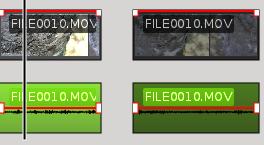
\includegraphics[width=0.38\textwidth]{images/splited}

  \end{center} \vspace{-20pt} \caption{Spliting} \label{Yes}

  \vspace{-10pt}

\end{wrapfigure}

La technique du decoupage de clip permet de diviser un footage en
plusieurs parties afin de pouvoir les utiliser de manière indépendante.

\paragraph{}

\paragraph{Unlinking de la piste audio et de la piste vidéo}

\begin{wrapfigure}{r}{0.6\textwidth}

  \vspace{-20pt} \begin{center}

  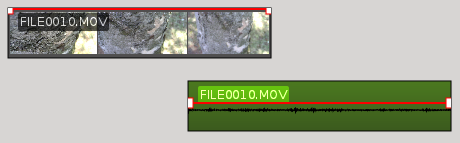
\includegraphics[width=0.38\textwidth]{images/unlinked}

  \end{center} \vspace{-30pt} \caption{Unlinking} \label{Yes}

  \vspace{-10pt}

\end{wrapfigure}

Le fait de ``de-lier'' les clips permet de gérer de manière
desynchronisée le son et la video.

\paragraph{Gestion des "in point" et  "out point" des clips} %Should that
                                                         %be translated?NON

  Permet de définir la partie d'un footage à utiliser dans le montage
  final. Cela permet donc de redéfinir la longueur d'un clip dans la
  timeline, en ne jouant pas le debut ou la fin de celui-ci.

\paragraph{}

\paragraph{Notion de layer}

\begin{wrapfigure}{r}{0.6\textwidth}

  \begin{center}

    \vspace{-20pt} 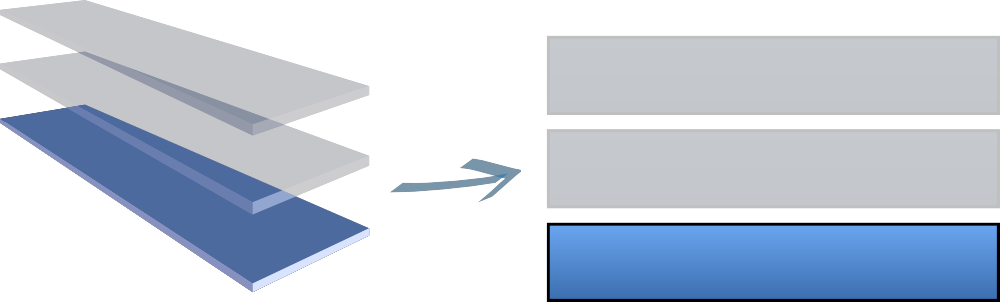
\includegraphics[width=0.38\textwidth]{images/layers}

  \end{center} \vspace{-20pt} \caption{Les layer} \label{Yes}

\end{wrapfigure}

La notion de layer est essentielle dans l'édition video avancée dans
la timeline : mixer plusieurs sources et ajouter des titres dépend de
cette fonctionnalité. Afin de comprendre, il est plus simple de faire
la comparaison avec de la peinture sur verre : on superpose plusieurs
vitres les unes au dessus des autres, chacune de ces vitres représentant
un layer. %C'est la superposition des dessins de chcune des plaques qui 
%va nous révéler le résultat final. De plus, il existe dans les layers une
notion d'opacité , %ce qui permet d'atténuer ou de révéler intégralement
%les dessins des plaques inférieures. 
\newpage

\section{Définition du marché par segment}

\paragraph{}

Dans un premier temps, nous allons définir et analyser les différents
formats de productions audiovisuelles professionnelles.  Nous avons
interviewé %un certain nombre de monteurs professionnels, afin de %lister leurs
besoins, (annexes 1) et en essayant de couvrir le maximum de champs de
l'édition vidéo. Nous avons pu récolter des informations provenant
de monteurs de clips vidéos, de courts métrage, de publicités et
de reportages.

\paragraph{}

La littérature dans la matière (En particulier
\cite{WorldVideoNonlinearEditingMarket}) nous propose de faire une nette
distinction entre  les deux segments du marché que sont:

\begin{itemize} \setlength{\itemsep}{2mm}

  \item {le monde du contenu post-produit: il s'agit de contenu dont la
  qualité de
    montage final est très importante. Celui-ci peut être de courte
    durée, tels que les clips vidéos ou publicités, %ou bien de longue
    durée, tels que les films% ou les séries télévisées. Mais il
    faut toutefois faire une différence entre ces derniers puisque la
    qualité du rendu final des films implique d'autres standards en
    terme de montage}

  \item {le monde de la production diffusée: il s'agit du contenu
  retransmis à la fois,
    sur internet, et sur les chaînes de télévisions et dont la
    création et la retransmission rapide impliquent des moyens spéciaux
    %qui permettent de créer et retransmettre le contenu dans un
    temps restreint, voir en direct.}

\end{itemize}

\paragraph{}

Certes les deux mondes ont des contenus différents, mais surtout
ils ont des contraintes différentes, ce qui implique des divergences
importantes en terme de besoin de fonctionnalités. Nous allons donc
nous intéresser à ces deux domaines et découper notre analyse à
partir de cette distinction. Tout d'abord, nous nous intéresserons aux
fonctionnalités logicielles nécessaires à la production de contenu
post-produit, par la suite, nous analyserons les besoins intrinsèques
à la production de contenu visant le monde de la vidéo diffusée. Puis
nous essayerons de voir où se situe la frontière entre ces deux mondes
afin de pouvoir par la suite nous rendre compte de ce que l'investissement
sur ces marchés implique pour les logiciels de montage vidéo libres.

\paragraph{Le monde du contenu post-produit}

\subparagraph{}

Le monde du contenu post produit est assez vaste, au premièr abord
il peut apparaître comme étant tout le contenu qui n'est pas diffusé
instantanément. Dans les faits, la distinction est plus complexe, et il
s'agit d'œuvres audiovisuelles dont le temps de post production n'est
pas un critère de première d'importance pour le choix des moyens mis
en place sur ce sujet.

\subparagraph{}

De ce fait, les formats suivants peuvent être considérés comme étant
post produits:

\paragraph{Les courts métrages}

\subparagraph{}

Les courts métrages concentrent %une histoire en moins de 35 minutes. Ils
sont donc soumis à des contraintes importantes.%Ils répondent
à une exigence de concision et il est donc intéressant de se poser la
question pour savoir si dans ce genre d'œuvre les monteurs utilisent
des techniques qui permettent de les rendre plus dynamiques et si des
fonctionnalités spéciales sont utilisées dans ce but.

\subparagraph{}

Dans la production de ce type d'œuvre, les interviews nous ont %révélé
%des fonctionnalités indispensables
telles que: \begin{itemize} \setlength{\itemsep}{2mm}
  \item{Transition (fading en priorité)} \item{Effets basiques %(par exemple
  %le passage en noir et blanc)\ldots} \item{Time remmaping} \item{Retouche
  des couleurs} \item{Création et ajout de génériques}
\end{itemize}

\paragraph {Les publicités}

\subparagraph{}

La publicité peut s'apparenter au court métrage puisqu'il s'agit de
création courte et généralement dynamique mais dont %l'objectif est différent.
Pour atteindre %cet objectif (attirer des consommateurs),
les monteurs utilisent des techniques spéciales mais les fonctionnalités
du logiciel nécessaires restent identiques à celles du court métrage.

\subparagraph{}

En revanche, la qualité du rendu est très importante%: ainsi des
logiciels spécialisés sont fréquemment utilisés afin de créer le
contenu (audio, effets, images\ldots).

\paragraph {Les clips vidéos}

\subparagraph{}

Le clip vidéo est un contenu visuel qui a pour but d'illustrer une
musique. Ce type de vidéos utilise souvent beaucoup d'effets spéciaux,
et demande à priori une très grande précision au niveau de la
synchronisation entre le son et l'image. La track audio dans de telle
production sera de préférence effectuée avec un logiciel dédié
à cet effet. Pour résumer, les fonctionnalités nécessaires sont:
\begin{itemize} \setlength{\itemsep}{2mm}
  \item{Création de titres complexes (Titre en mouvement, etc\ldots)}
  \item{Ajout de titres} \item{Ajout d'effets} \item{Utilisation avancé
  des keyframes} \item{Time remapping}
\end{itemize}

\paragraph {Les films}

\subparagraph{}

La production cinématographique bénéficie de budgets beaucoup plus
élevés. %Les techniques employés dans le cadre de la post production
sont plus complexes et permettent de %gérer avec soin la qualité
du rendu.

\subparagraph{}

Il n'a pas été possible d'interviewer de monteur de film jusqu'à
maintenant, mais le livre ``The technique of film and video editing,
History, Theory, and Practice'' \cite{TheTechniqueOfFilmAndVideoEditing}
est un bon point de départ pour comprendre le montage cinématographique
et la très grande influence qu'il a sur les autres types de productions
audiovisuelles. On peut considérer le film comme étant une oeuvre
audiovisuelle par excellence. %FIXME formulation pourri

\subparagraph{}

Dans le monde du cinéma, le logiciel de montage vidéo est l'un des
logiciels parmi un système connecté de logiciel de post production. Des
spécialistes de différents domaines créent les parties du film,
et le monteur a pour mission de lier tout ces éléments au travers du
logiciel de montage. Les logiciels de post production sont entre autres:

\begin{itemize} \setlength{\itemsep}{2mm}

  \item{Éditeur de son}

  \item{Création d'effet}

  \item{Retouche d'image}

  \item{Création d'animation}

  \item{\ldots}

\end{itemize}

\subparagraph{}

Les logiciels à visée professionnelle ne sont donc pas forcément
utilisables dans le monde de la création cinématographique. Il
conviendra de faire une réelle différence entre ces deux univers du
montage vidéo.

\subparagraph{}

Ce qui résulte du fait que le logiciel de montage vidéo à proprement
parler ne demande pas vraiment de fonctionnalités très évoluées, la
base de l'édition et la possibilité d'organiser l'immense quantité
de Footages de manière efficace semblent être éléments clefs dans
ce domaine.(Phrase confuse à repréciser)%PHRASE TRES CONFUSE. Les autres logiciels de post
production sont bien évidemment aussi nécessaires afin de permettre de
faire le montage de films.%Ce document n'a pas pour but de détailler ces autres logiciels. 

\subparagraph{}

Une autre caractéristique de la production cinématographique, qui
%est une conséquence directe de l'impératif de qualité
irréprochable, %réside dans le fait
que les logiciels de montage doivent permettre de
visualiser chaque image du film de manière très précise (le montage
de film se fait dans certain cas en choisissant chaque image depuis un
tableau de frames \index{frame}).

%FIXME, faudrait plus détailler ici? Qui doit répondre ? Ton maitre
de stage ? Toi?

\subparagraph{}

Bien que ne demandant pas vraiment de fonctionnalités très avancées,
la création de film a des besoins assez évoluées en ce qui concerne
le logiciel de montage: \begin{itemize} \setlength{\itemsep}{2mm}
  \item{Organisation très avancée des Footages} \item{Création et
  ajout de générique} \item{Passerelles avec le reste des logiciels
  de post production} \item{Preview de chaque frame dans le détail}
\end{itemize}

%TODO essayer de trouver des monteurs de films!

\paragraph {Les séries télévisées}

\paragraph{}

Le niveau de qualité des séries télévisées n'étant pas aussi élevé
que pour le montage des films, les traitements sont la plupart du temps
réalisés directement dans le logiciel de montage même. Cela implique
un nombre de fonctionnalités plus important avec comme nécessité:
\begin{itemize} \setlength{\itemsep}{2mm}
  \item{Création et ajout de titre} \item{Création et ajout de
  générique} \item{Retouche des couleurs}
\end{itemize}

\paragraph {Les documentaires}

\paragraph{} Le documentaire est en général assez sobre en terme de
montage. %Il réside en général dans le logiciel de montage,
mais ne demande pas de fonctionnalités spéciales. % Les 
fonctionnalités utilisées pour produire ce type d'œuvre sont:
\begin{itemize} \setlength{\itemsep}{2mm}
  \item{Création et ajout de titre} \item{Création et ajout de
  génériques} \item{Retouche des couleurs} \item{Utilisation
  des keyframes} \item{Transition smpte\glossary{name={smpte},
  description={Society of Motion Picture
    and Television Engineers, est une association internationale,
    située aux É.-U., et composée d'ingénieurs. Elle développe
    des standards vidéos (elle en a déjà plus de 400 à son actif),
    qui sont utilisés par exemple par la télévision, ou le cinéma
    numérique (Source: http://fr.wikipedia.org/)}} \index{SMPTE}}
\end{itemize}

\paragraph{Le monde du contenu diffusé}

\paragraph{}
%JE NE VOIS PAS DE DEFINITION
La plupart du contenu post produit est par la suite diffusé,
la différence que l'on fait ici entre ces deux types de production
réside dans le temps de la post production.  Dans le cas des journaux
télévisés, émission de télé, la post production est soit totalement
inexistante (dans le cas du direct), soit très courte, dans le cadre
de reportages, jeux télévisés et autres types de production visant
spécifiquement la télévision.

\paragraph {Les émissions télévisées}

\paragraph{}

% Suivant leur mode de production, les émissions de télévision peuvent%
%être classées soit dans le contenu post-produit
%soit dans le contenu diffusé. %Elles sont en
général diffusées très rapidement après la création du contenu
(si ce n'est en direct)% et c'est la raison pour laquelle nous les considérons
%comme du contenu
diffusé. De plus le fait qu'elles soient produites exclusivement pour
la diffusion (aucune commercialisation matérielle n'en est faite),
cette classification paraît naturelle.

Du fait de leur temps de production très réduit, les principales
fonctionnalités en terme de logiciel de montage sont: \begin{itemize}
\setlength{\itemsep}{2mm}
  \item{Fonctionnalité de template qui permet d'avoir un cadre général
  de montage de
    présentations, au moment voulu et ainsi faire le montage en direct}
  \item{Titres}
\end{itemize}

\paragraph{}

Bien évidemment, dans le cadre de la création de template,
les transition ``smpte''\index{SMPTE} et les effets simples sont
généralement utilisés. Mais il n'est pas rare que les template à
proprement parler ne soient pas créés dans le logiciel de montage,
mais plutôt dans d'autres logiciels de création de contenu audiovisuel.

\paragraph {Évènements spéciaux (sportif, d'actualité\ldots)}

\paragraph{}

%En principe ce type de production audiovisuelle n'est %pas 
post-produit. Il s'agit de production instantanée, et pour ce type
de contenu, l'outil de montage non linéaire doit permettre de donner
une impression de contenu post-produit alors qu'il n'en est rien. Les
fonctionnalités nécessaires sont assez similaires à celles dont on
aurait besoin pour produire des émissions de télévision.

\subparagraph{}

De plus, l'acquisition étant aussi fait en direct, il doit être possible
d'intégrer le logiciel du montage dans le système de capture d'image
et de son.

De même que pour les émissions de télé, les template sont
généralement produits avec des logiciels dédiés à cet effet.

\subsection{Analyse des fonctionnalités communes}

\paragraph{}

On s'aperçoit donc que de nombreuses fonctionnalités sont communes aux
différents types d'œuvres. Il convient de détailler chacune de ces
fonctionnalités afin de nous rendre compte de ce qu'elles impliquent
en terme de logiciel de montage.

\paragraph{Création et ajout de titre}

\paragraph{}

Cette fonctionnalité est utilisée dans la création de plusieurs types
de contenu: \begin{itemize} \setlength{\itemsep}{2mm}
  \item {Séries télévisés} \item {Documentaires} \item {Clips vidéos}
\end{itemize}

\paragraph{}

Bien que cette fonctionnalité est utilisée dans différents
types de contenu, %le logiciel sera le résultat
%de différents paramètres. Par exemple,
dans une série télévisée %le travail sur les titres sera
assez limité: on aura souvent une vidéo en arrière-plan et un titre que
fera un fondu arrière. %En revanche dans le cadre de clips vidéo, on verra
%fréquemment le titre en mouvement sur le rythme de la
musique par exemple. %Il est nécessaire de tout mettre en oeuvre pour répondre 
%à la diversité de ces beoins
mais il sera plus difficile aussi bien en terme de backend qu'en terme
d'interface utilisateur de répondre aux besoins les plus spécifiques.

\paragraph{Création et ajout de générique}

\paragraph{}

La création de générique est une fonctionnalité indispensable,
à laquelle de nombreux monteurs (en particulier professionnels)
font appel. Cette fonctionnalité en terme de backend est similaire à
celle des titres puisqu'il s'agit ni plus ni moins d'ajouter du texte
au dessus d'un fond qu'il soit animé ou non. Mais en terme d'interface
utilisateur, \glossary{name={Interface Utilisateur}, description={User
Interface, il s'agit du terme  très largement employé pour définir
l'interface utilisateur, en général graphique ou GUI}}, il s'agit
de deux fonctionnalités différentes puisque par définition, le
générique est un texte qui défile dans une très grande majorité
des cas, de haut en bas.

\paragraph{}

Cette fonctionnalité est l'une des plus basiques si l'on veut pouvoir
répondre aux besoins des professionnels. Elle est utilisée dans la
plupart des créations vidéo et doit être à priori standardisée et
simple à utiliser dans l'interface utilisateur afin que la mise en place
des génériques (déjà écrits) soit effectuée de manière simple et
rapide par les monteurs.

\paragraph{Gestion des Keyframes:}

\paragraph{}

Les keyframes sont utilisées dans bien des domaines, mais dans beaucoup
de cas, elles sont utilisées avec parcimonie. Elles permettent dans une
vidéo, d'animer les propriétés d'éléments ajoutés par le monteur
(effets, texte, etc\ldots). Il apparaît donc nécessaire d'avoir une
gestion minimale des keyframes, en particulier pour une gestion fine
des couleurs, mais leur utilisation est rarement vraiment avancée.

\paragraph{}

Dans la création de clips en particulier, afin de dynamiser la vidéo,
les monteurs utilisent de manière intensive les keyframes.

\subsection{Fonctionnalités spécifiques} %Ils ? que dans %FIXME %les
faits, les fonctionnalités utilisées sont assez similaires bien que
%les œuvres finales soient totalement différentes.

\paragraph{}

Quelques fonctionnalités sont apparues comme vraiment propres à la
création d'un type d'oeuvre en particulier.

\paragraph{Visualisation image par image:}

\begin{wrapfigure}{r}{0.5\textwidth}
    \begin{center}
      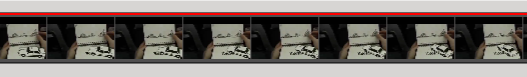
\includegraphics[width=0.48\textwidth]{images/frameByFrame}
    \end{center} \caption{Visualisation frame par frame} \label{Yes}
\end{wrapfigure}

Dans le cadre de la création de film, la prévisualisation de
chaque frame de manière précise semble être une fonctionnalité
essentielle.% Cela signifie que le logiciel de montage doit permettre
de voir de manière simple chaque frame des vidéos présentes dans
la timeline. Cette fonctionnalité est aussi utile dans le cadre de
la création d'autres oeuvres, mais %elle est indispensable dans le cas de
films, %permettant ainsi de s'assurer de la qualité du résultat. En effet, lors de
la création d'un film, chaque frame doit être contrôlée%.
%Dans d'autres types d'œuvres, les exigences %et les moyens étant moins élevées
%, une telle fonctionnalité n'est pas indispensable.

\paragraph{Gestion avancée des Footages}

\paragraph{}

Dans le cadre de productions longues, un des problèmes auquel doit
répondre de manière satisfaisante le logiciel d'édition est la gestion
et la classification des Footages. % C' est en particulièrement vrai pour
les films et les séries télévisées.  Dans ces types de productions le
nombre d'heures de Footages peut être très grand, et le monteur doit
dans un premier temps établir une classification des Footages. Le
logiciel de montage doit, pour répondre aux besoins des monteurs,
permettre de les ordonner de manière précise et bien pensée.

\paragraph{Intégration dans un écosystème de logiciel de post
production}

\paragraph{}

Dans le cadre de création de films en particulier, on constate %
% que le logiciel de montage doit s'intégrer dans
l'écosystème de logiciel de post production. %C'est généralement 
possible si ce logiciel de montage respecte les quelques standards de
la post production d'oeuvre audiovisuelle comme par exemple le Material
eXchange Format \glossary{name = {MXF}, description={Material eXchange
Format ou MXF est un conteneur utilisé par les professionnels pour les
données audio et vidéo numériques. Il s'agit d'un format défini par
des standards de la SMPTE\index{SMPTE}. (Source: wikipedia)}} \index{MXF}

\paragraph{Time remapping}

\paragraph{ }

Le time remapping, comme précédemment indiqué, est particulièrement
utilisé dans la création de contenu court. Il permet d'accélérer,
où ralentir une partie d'un clip pour le rendre l'œuvre la plus
dynamique possible.

\paragraph{Gestion des templates}

\paragraph{ }

La création de contenu non post produit demande des fonctionnalités
particulières. La fonctionnalité qui apparaît comme clé pour répondre
aux besoins liés à ce type de produit est la création de template. Par
exemple la création de journaux télévisés ou autres évènements
sportifs %
demande une gestion avancée de ``moule``, ou template, qui permet de
simplement lier les contenus des différentes caméras à un moment
donné de la retransmission.

\paragraph{ }

Cette fonctionnalité n'est pas exclusivement utilisée dans la création
de contenu en direct, mais elle est très largement utilisée dans tout
ce qui est contenu destiné à la télévision.

\paragraph{} \paragraph{}

En conclusion, on a constaté que le champ de fonctionnalité est vaste,
la plupart de ces fonctionnalités sont génériques et leur utilisation
est,par conséquent, commune à différents types d'œuvres.En revanche
ce qui varie particulièrement  est la finesse d'implémentation et le
niveau d'utilisation qu'en fait le monteur.

\newpage \section{Comparaison des principaux logiciels présents sur le
marché de
  l'édition vidéo professionnel, et analyse des manques et risques
  du marché}

\paragraph{}

Il conviendra d'analyser précisément les logiciels existants, qu'ils
soient propriétaires ou libres. Cette partie a pour but de rendre compte
de l'état actuel du marché des logiciels d'édition vidéo qui ont pour
principal public les professionnels. Cette étude portant principalement
sur les logiciels libres, ceux-ci seront évidemment inclus dans cette
analyse bien que l'on puisse considérer que à cause de leur manque de
maturité, ils n'y aient pas totalement leur place.

\paragraph{}

Dans cette optique, on analysera les points clés des logiciels.
Tout d'abord on comparera les fonctionnalités des logiciels, la
manière dont elles sont gérées, et on essayera d'avoir l'avis de
professionnels sur ces fonctionnalités et leur implémentation dans les
différents logiciels. Ensuite on regardera le prix de ces logiciels,on
verra en quoi cela peut être un argument de poids pour les logiciels
libres et leur éventuelle prise de part de marché. Par la suite nous
nous concentrerons sur la documentation, livres et autres tutoriels
disponibles pour ces différents logiciels, et %nous verrons quels supports
sont offerts aux professionnels pour ces logiciels.

\subsection {Historique du marché}

Les tout premiers logiciels d'édition non linéaire ont vu le jour dans
le début des années 70.  A cette époque les solutions de stockages
de données étant très limitantes, les premiers logiciels de montage
vidéo non linéaire effectivement utilisables ont vu le jour en
1989, ceux-ci étaient basés sur les disques durs pour ce qui est du
stockage. C'est cette année là que ``Editing Machines Corp.'' et Avid
ont mis sur le marché les logiciels de montage vidéo non linéaire
ainsi que le matériel qui permettait son utilisation. Une fois de plus,
les limitations en terme de stockage de données (accès limité à
50 Gigabytes à la fois maximum), rendait l'utilisation des systèmes
de montage non linéaire inutilisables dans le domaine du cinéma,
et même dans de nombreux cas de la télévision. C'est en 1992 que
cette limitation a été surmontée, il était alors possible d'accéder
jusqu'à 7 Terabytes de données à la fois, ce qui rendait envisageable
le montage de production longue de manière informatique. C'est en
1993 que Avid prend avantage de cela et s'impose comme leader mondial,
remplaçant les équipements de montage de pellicules 35mm de toutes
les principales maisons de production cinématographiques dans le
monde. Avid a été le leader incontesté du marché de l'édition
professionnel jusqu'en 2003, date à laquelle Final Cut Pro a été
considéré comme une bonne alternative à Avid par les grands acteurs
de l'édition vidéo professionnel.

\subsection{Définition des plus grands acteurs du marché}

\paragraph {Logiciels commerciaux}

\subparagraph{Avid Media Composer:}

Leader historique du marché du logiciel de montage non linéaire
professionnel. Il s'agit du produit phare de Avid Technology publié en
1989. Depuis, ce logiciel a joué un rôle essentiel dans %le développement
de ce marché.

\subparagraph{Avid Symphony:}

Evolution de Avid Media Composer, il s'agit d'une version plus complète
en terme de fonctionnalités qui a pour but de répondre aux besoins
des monteurs de productions longues tels que les documentaires et les
séries télévisées.

\subparagraph{Final cut pro:}

Logiciel de montage intégré dans la suite de logiciels de
post-production de Apple, Final Cut Studio. Il s'agit d'un logiciel
de montage orienté à la fois professionnel et création de film. Il
est de nos jours très utilisé et est devenu l'un des leaders mondial
du marché.

\subparagraph{Adobe Premiere Pro:}

Logiciel de montage de la suite Adobe Creative suite, il s'agit du
logiciel d'édition vidéo à visée professionnelle de Adobe System. Il
est à la fois adapté pour la création de contenu diffusé, mais aussi
de contenu post produit

\paragraph {Logiciel en cours de libération:}

\subparagraph{lightworks:}

Logiciel de montage actuellement commercial, très puissant,
et offrant des fonctionnalités uniques, il permet de faire %paralèllement
la production diffusée et la création post-produit. %Ce produit est particulier 
%car ses créateursont décidé
de libérer le code source
\cite{TheLightworksOpenSourceProjectStartHere}, et ainsi  de créer une
communauté de développeurs pour en faire un projet de logiciel libre.

\paragraph {Logiciels libres:}

\subparagraph{Cinelerra:}

Logiciel de montage et de compositing libre développé principalement
par la société Héroïne \footnote{Heroine: http://heroinewarrior.com/}
et intégré par la société LMA\footnote{LMA: http://lmahd.com/}. Il
s'agit d'un logiciel de montage non linéaire avec de très nombreuses
fonctionnalités. Principalement créé pour le création de contenu
diffusé, il permet aussi de répondre aux besoins de la production
de contenu post-produit. Il s'agit du seul logiciel libre utilisé en
milieu professionnel.

\subparagraph{Kdenlive:}

Logiciel de montage libre s'intégrant dans la suite logicielle de
l'interface graphique KDE.  Ce logiciel de montage est assez complet et
peut répondre aux besoins des monteurs de contenu post-produit.

\subparagraph{PiTiVi:}

Logiciel de montage libre encore basique mais en plein développement.
Ce logiciel a pour but de répondre aux besoins du plus grand nombre,
et en particulier à ceux des professionnels de la création de contenu,
qu'il soit post produit ou non.


\subsection{Fonctionnalités}

\paragraph{}

<<<<<<< Other changes
Tout d'abord, il convient de voir quelles fonctionnalités existent chez
les différents acteurs du marché. Afin d'analyser ces fonctionnalités,
afin de faciliter la lecture et avoir une vision globale de ce qui
ce fait, le diagramme en toile d'araignée suivant a été créé.
D'après les interview et l'analyse précédemment faites, les axes
suivants ont été choisis: \begin{itemize} \setlength{\itemsep}{2mm}
=======
Tout d'abord, il convient de voir quelles fonctionnalités
existent chez les différents acteurs du marché. Afin d'analyser ces
fonctionnalités, afin de faciliter la lecture et avoir une vision
globale de ce qui ce fait% nous avons fait une représentation sur 
%un diagramme en toile d'araignée.  
D'après les interview et l'analyse précédemment
faites, les axes suivants ont été choisis:
\begin{itemize} \setlength{\itemsep}{2mm}
>>>>>>> Your changes
  \item{Gestion des formats de fichiers} \item{Integration dans
  un écosystème de post production} \item{Gestion des template}
  \item{Gestion des footage} \item{Colorimétries} \item{Effets}
  \item{Transitions} \item{Support multi-platform}
\end {itemize}

\paragraph{} Dans le schéma suivant le niveau et la qualité
d'implémentation a été prise en compte. Les retours utilisateurs
ont aussi une place importante dans cette évaluation. La plupart de
ces évaluations portent sur des données non quantifiables, pour cette
raison, aucune échelle précise n'est donnée.  Par exemple, l'ergonomie
ne peut être quantifiée, seul le ressenti des utilisateurs peut être
analysé, et c'est ce travail qui a été effectué.

\begin{figure} [H]

  \begin{center}

    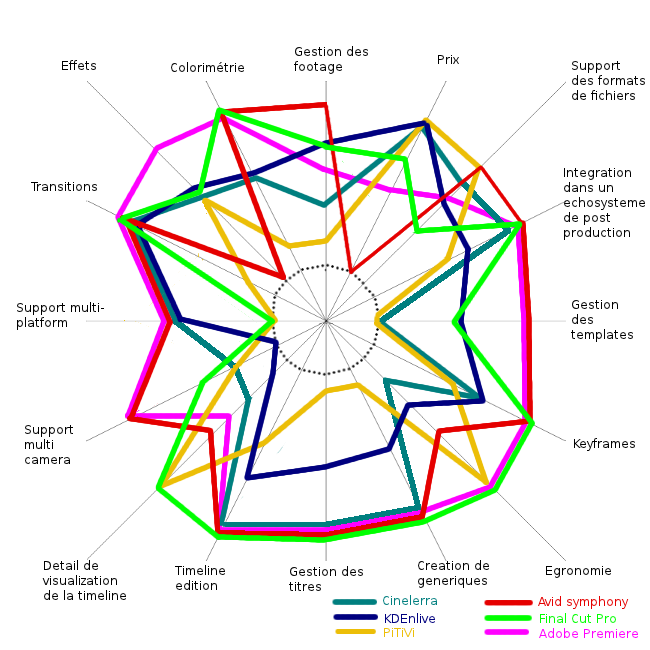
\includegraphics[width=0.9\textwidth]{images/spiderDiagramFeaturesComparision}

  \end{center}

  \caption{Comparaison des fonctionnalités des logiciels leaders sur
  le marché}

  \label{Yes}

\end{figure}

\paragraph {}

<<<<<<< Other changes
Ce schéma nous permet de très facilement expliquer le faite que les
seul logiciel libre cinelerra est une pas une place sur ce marché,
leur lacunes de PiTiVi et Kdenlive en terme de fonctionnalité rend leur
utilisation impossible en milieu professionnel. Dans la seconde partie
nous nous attarderons plus sur chacun de ces trois logiciels libres
afin de nous rendre compte quel sont les fonctionnalité manquante,
et ceux par format de contenu.
=======
Ce schéma nous permet % d'expliquer très facilement que les
logiciels libres %n'ont pas de place sur ce marché: leurs lacunes en
terme de fonctionnalité rend leur utilisation impossible en milieu
professionnel. Dans la seconde partie nous nous attarderons plus sur
chacun de ces trois logiciels libres afin d%'analyser quelles
sont les fonctionnalités manquantes, et %????ceux par format de contenu.
>>>>>>> Your changes


\newpage

\section{Visions du marché par les professionnels du montage}

\paragraph{L'importance de la position du logiciel sur le marché}

\subparagraph{} En ce qui concerne le choix du logiciel de montage dans
<<<<<<< Other changes
une entreprise, la connaissance qu'ont les monteurs du logiciel qu'ils
utilisent est essentiel.  C'est pour cela, que dans de nombreux cas,
le premier facteur de choix, est la part de marché de ce logiciel sur
le marché de l'édition vidéo. En effet, les différentes industries
veulent être sûres qu'il est possible de trouver de la main d'oeuvre
compétente sur le logiciel qu'elle utilise.  Mais ce n'est pas seulement
la disponibilité de personnes compétentes qui est importante, il
est également indispensable que ces dernières puissent se former
et qu'elles aient accès facilement aux informations concernant les
nouvelles résolutions des problèmes posés par un logiciel au travers
des différentes versions.
=======
une entreprise, la connaissance qu%e les monteurs ont du logiciel qu'ils
utilisent est essentiel.  C'est pour cela que dans de nombreux cas
le premier facteur de choix est la %position de ce logiciel
sur le marché de l'édition vidéo. En effet, les différentes
industries veulent être sûres qu'il est possible de trouver de la
main d'oeuvre compétente sur le logiciel qu'elle utilise.  Mais ce
n'est pas seulement la disponibilité de personnes compétentes qui
est importante, il est également indispensable que ces dernières
puissent se former et qu'elles aient accès facilement aux informations
concernant les nouvelles résolutions des problèmes posés par un
logiciel au travers des différentes versions.
>>>>>>> Your changes

\subparagraph{} Comme l'a souligné M. Faure lors de son interview
(annexe 3), dans son cas, il ne serait pas envisageable de changer de
logiciel à moins que le marché n'évolue. C'est à dire que l'un des
critères de choix dans son cas est la position de tel logiciel sur
le marché. Cela est principalement une question de crédibilité, et
donc afin d'éviter la prise de risque, les professionnels préfèrent
prendre la référence du marché.

\subparagraph{}

Mais cela est principalement vrai dans les structures de taille moyenne.
Dans le cadre de petits structures, comme l'a souligné M. Veri
<<<<<<< Other changes
(annexe 1) durant son interview, il serait plus probable que afin de
se différencier, d'une manière où d'une autre de la concurrence, de
choisir un logiciel différent de celui de référence. Bien évidemment,
cela à la condition qu'il réponde convenablement à leurs besoins
et permette de satisfaire les demandes de leurs clients. Dans son cas,
M. Veri estime qu'un tel logiciel n'existe pas et que la référence du
marché (Final Cut Pro) est en réalité la meilleure option.
=======
(annexe 1) durant son interview, il serait %plus logique, 
%dans un souci de se différencier de ses concurrents,
de choisir un logiciel différent de celui de référence. Bien
évidemment %ce logiciel devra répondre convenablement
à leurs besoins et permette de satisfaire les demandes de leurs
clients. Dans son cas, M. Veri estime qu'un tel logiciel n'existe pas
et que la référence du marché (Final Cut Pro) est en réalité la
meilleure option.
>>>>>>> Your changes

\paragraph{Dépendance vis-à-vis du créateur}

\subparagraph{}

<<<<<<< Other changes
L'un des point qui ressort des interviews, est que pour les professionnels
du montage (comme dans beaucoup de domaines liés aux nouvelles
technologies), le changement de l'expérience utilisateurs au travers
des versions est quelque chose de très appréhendé?. Un bon exemple
de ce fait est la dernière version de Final Cut Pro, qui a été très
négativement critiquée \cite{FinalCutProXReviews} : Apple a décidé
de changer le workflow \index{workflow} des professionnels de l'édition
vidéo dans la dernière monture de leur logiciel phare de ce secteur,
et cela a très mal été perçu par les professionnels. Toutefois pour
M. Faure, ce problème n'est pas trop grave, puisqu'il considère que dans
le cas où la transition à cette nouvelle version soit top compliquée
(coute trop cher que la formation du personnel soit trop onéreuse,
et fasse perdre trop de temps), ils ont toujours l'option de garder,
la version courante.  Mais cela n'est valable que sur le court terme,
puisqu'il n'est pas envisageable, pour des raison de sécurité et de
support, d'utiliser de manière commerciale un logiciel non maintenu
et non supporté par l'entreprise éditrice. Pour M. Veri en revanche,
cela pose aussi un problème important, et ayant lui même utilisé
cette nouvelle monture, il considère qu'il serait préférable pour
son entreprise de trouver une alternative.

\subparagraph{}

Dans le cadre de structures importantes, la dépendance vis-à-vis des
éditeurs est parfois considérée comme quelque chose de dangereuse,
qu'il faut éviter au maximum. Par exemple, Dreamworks Picture, a décidé
de créer et de maintenir leur propre suite logiciel \cite {Dreamworks}
de poste production. Leur principal objectif  est de garantir que
les logiciels qu'ils utilisent répondent à leurs besoins précis,
d'en maitriser son leur évolution et ainsi de ne pas dépendre d'un
éditeur externe. De plus, afin de garantir leur son indépendance, cette
entreprise a décidé d'utiliser Linux comme système d'exploitation
(distribution Red Hat), ce qui leur lui garantit un grande liberté. De
plus, cette entreprise a décidé d'employé la partie ``Dreamworks
Animations'' est cliente de ma société LMA, ce qui signifie que
très probablement celle-ci utilise Cinelerra dans leur processus de
post-production. De même les société de télévision Française TF1
et Canal+ sont cliente de cette même entreprise, ce qui montre bien
que Cinelerra est utilisé de manière professionnel. Bien que d'après
M. Faure, TF1 semble abandonner petit à petit Cinelerra au profit de
Final Cut Pro.
=======
%Un souci important des professionnels du montage qui ressort des interviews
%est le changement de l'expérience utilisateur: l'arrivée d'une nouvelle 
%version est redoutée car elle demande un temps d'adaptation pour la maitriser.
%Ceci peut être illustré par la dernière version de Final Cut Pro, qui
a été très %critiquée \cite{FinalCutProXReviews}
: Apple a décidé de changer le workflow \index{workflow} des
professionnels de l'édition vidéo dans la dernière monture de leur
logiciel phare de ce secteur, et cela a très mal été perçu par
les professionnels. Toutefois pour M. Faure, ce problème n'est pas
trop grave, puisqu'il considère que dans le cas où la transition
à cette nouvelle version %s'avère compliquée (trop coûteuse, %
%formation du personnel trop onéreuse, perte de temps pour maitriser)
, %ils ont toujours avec Apple a toujours l'option de conserver la version
courante.  Mais cela n'est valable que sur le court terme, puisqu'il
n'est pas envisageable, pour des raisons de sécurité et de support,
d'utiliser de manière commerciale un logiciel non maintenu et non
supporté par l'entreprise éditrice. Pour M. Veri en revanche, cela
pose aussi un problème important, et ayant lui même utilisé cette
nouvelle %version, il considère qu'il serait préférable pour
son entreprise de trouver %QUOI?

\subparagraph{}

Dans le cadre de %structures importantes, la dépendance
vis-à-vis des éditeurs est parfois considérée %
%potentiellement dangereuse, et donc à éviter . Par exemple,
Dreamworks Picture, a décidé de créer et de maintenir leur propre
suite logiciel \cite {Dreamworks} de post production. %Leur
principal %objectif  est d'avoir la garantie que leurs logiciels 
%répondent bien à leurs besoins précis en maitrisant  leur
évolution %. Ils ne dépendent plus d' un éditeur externe et pour conforter cette
afin de garantir leur son indépendance, cette entreprise a décidé
d'utiliser Linux comme système d'exploitation (distribution Red Hat),
ce qui leur lui garantit un grande liberté. De même la société
de télévision Française TF1 a développé ses logiciels de post
production en interne, mais, elle semble les abandonner petit à petit
au profit de Final Cut Pro.
>>>>>>> Your changes

\newpage

\section {Bilan}

\paragraph { }

Nous constatons donc, que, bien que le marché soit vaste et varié,
à l'heure actuelle, seuls quelques logiciels permettent de répondre
aux besoins de la grande majorité des utilisateurs.

\paragraph{}

Les professionnels sont plutôt satisfaits par les logiciels commerciaux
existants dont ils disposent, mais il existe des limitations dues au
fait que ces logiciels, sont des logiciels fermés, et édités par une
seule entreprise qui décide de ce dont les utilisateurs ont besoin des
besoins des utilisateurs. Partant de ce constat on peut se demander
si l'utilisation de logiciels ouverts et édités par de nombreuses
entreprises, pourraient prendre une place encore plus importante sur le
marché, en offrant de nouvelles perspectives pour les acteurs du marché
du montage vidéo. Les points suivants peuvent être considérés comme
des points importants sur un marché fermé, et contrôlé par un nombre
très restreint d'entreprises:

\paragraph{Plus grande autonomie vis-à-vis de la société éditrice
(développeur/designer):}

  \subparagraph{ }

    Grâce à l'utilisation de logiciel libre, il est possible de
    garantir, et maintenir le logiciel en interne tout en profitant
    du fait que des personnes externes à l'entreprise, d'une part
    le développent, et d'autre part, le connaissent. Cela a pour
    conséquence que les coûts sont très largement réduits en
    comparaison à ce qui est actuellement pratiqué chez Dreamworks et
    TF1 par  exemple.

\paragraph{Possibilité collaboration et communication avec les
développeurs:}

  \subparagraph{}

  Le développement des logiciels libres étant en principe fait
  publiquement, les utilisateurs (entreprises qui font le montage
  vidéos) peuvent voir l'évolution du logiciel au fur et à mesure
  de sa progression. Cela leur permet aussi de donner leur avis sur les
  directions à prendre.

\paragraph{Réduction de coût:}

\subparagraph{}

Comme l'ont souligné  M. Veri et M. Hachemi au cours de leur interview,
dans le cadre de petites structures c'est un argument important.
En effet,  actuellement les frais liés à l'achat de licences pour
les logiciels de montage constituent une charge financière importante
compte tenu des prix de ces licences. L'utilisation de logiciel libre
permet donc, dans la très grande majorité des cas, de réduire
considérablement les coûts de montage, puisque le code source est
libre d'accès.

\paragraph{Possibilité d'adaptation aux besoins précis de l'entreprise:}

\subparagraph{}

L'ouverture du code et sa mise à disposition à tous ouvre la
possibilité d'effectuer des adaptations dans le core même du logiciel,
et ainsi de développer des versions spécialement adaptées aux besoins
de l'entreprise utilisatrice.

\subparagraph{}

Alors que dans le cadre de projets commerciaux,  le développement et
l'adaptation de différentes versions ne sont faites que par l'entreprise
éditrice. On peut cependant, même dans ce cadre-là, modifier, ajouter
des fonctionnalités grâce aux systèmes d'extension logicielle, mais
la flexibilité offerte par ce système reste limitée à ce que la
société éditrice veut bien mettre à disposition des développeurs
externes. (En terme d'API \index{API} \glossary{name={API}, description={
Une interface de programmation (Application Programming Interface
ou API) est une interface fournie par un programme informatique. Elle
permet l'interaction des programmes les uns avec les autres, de manière
analogue à une interface homme-machine, qui rend possible l'interaction
entre un homme et une machine}}.

\paragraph{}

On voit que des logiciel libre sont utilisés en milieu professionnel,
mais cela est un phénomène mineur. Les opportunités que ces logiciels
peuvent apporter au monde de la post-production professionnel étant
importants, il convient d'étudier le potentiel de ces logiciel dans
ce domaine.
